\documentclass[spec, och, otchet, hidelinks]{SCWorks}
% параметр - тип обучения - одно из значений:
%    spec     - специальность
%    bachelor - бакалавриат (по умолчанию)
%    master   - магистратура
% параметр - форма обучения - одно из значений:
%    och   - очное (по умолчанию)
%    zaoch - заочное
% параметр - тип работы - одно из значений:
%    otchet
%    referat    - реферат
%    coursework - курсовая работа (по умолчанию)
%    diploma    - дипломная работа
%    pract      - отчет по практике
%    pract      - отчет о научно-исследовательской работе
%    autoref    - автореферат выпускной работы
%    assignment - задание на выпускную квалификационную работу
%    review     - отзыв руководителя
%    critique   - рецензия на выпускную работу
% параметр - включение шрифта
%    times    - включение шрифта Times New Roman (если установлен)
%               по умолчанию выключен
\usepackage[T2A]{fontenc}
\usepackage[utf8]{inputenc}
\usepackage{graphicx}

\usepackage[sort,compress]{cite}
\usepackage{amsmath}
\usepackage{amssymb}
\usepackage{amsthm}
\usepackage{fancyvrb}
\usepackage{longtable}
\usepackage{array}
\usepackage{listings}
\usepackage{xcolor}
\usepackage[english,russian]{babel}
% Используется автором репозитория
%\usemintedstyle{xcode}
% Этот пакет включает в себя аналогичный Times New Roman шрифт.
% Необходим для успешной компиляции для UNIX-систем ввиду отсутствия TNR в нем.
% Можно использовать и для Windows.
\usepackage{tempora}

\lstset{%
	language=C,
	backgroundcolor=\color{gray!12},
	basicstyle=\ttfamily\small,
	keywordstyle=\color{blue},
	stringstyle=\color{blue},
	showstringspaces=false,
	captionpos=b,
	numbers=left,
	numberstyle=\footnotesize\color{gray},
	frame=TB,
	tabsize=2,
	morekeywords={procedure, then, begin, end}
}

\usepackage[colorlinks=false]{hyperref}

\graphicspath{{figures/}}

\newcommand{\eqdef}{\stackrel {\rm def}{=}}

\usepackage{stackengine}
\newcommand\xrowht[2][0]{\addstackgap[.5\dimexpr#2\relax]{\vphantom{#1}}}

\newtheorem{lem}{Лемма}

% % При использовании biblatex вместо bibtex
%\usepackage[style=gost-numeric]{biblatex}
%\addbibresource{thesis.bib}

\begin{document}

% Кафедра (в родительном падеже)
\chair{математической кибернетики и компьютерных наук}

% Тема работы
\title{Преобразователи кодов}

% Курс
\course{3}

% Группа
\group{331}

% Факультет (в родительном падеже) (по умолчанию "факультета КНиИТ")
%\department{факультета КНиИТ}

% Специальность/направление код - наименование
%\napravlenie{02.03.02 "--- Фундаментальная информатика и информационные технологии}
%\napravlenie{02.03.01 "--- Математическое обеспечение и администрирование информационных систем}
%\napravlenie{09.03.01 "--- Информатика и вычислительная техника}
%\napravlenie{09.03.04 "--- Программная инженерия}
\napravlenie{10.05.01 "--- Компьютерная безопасность}

% Для студентки. Для работы студента следующая команда не нужна.
%\studenttitle{Студентки}

% Фамилия, имя, отчество в родительном падеже
\author{Бородина Артёма Горовича}

% Заведующий кафедрой
\chtitle{доцент, к.\,ф.-м.\,н.} % степень, звание
\chname{С.\,В.\,Миронов}

%Научный руководитель (для реферата преподаватель проверяющий работу)
\satitle{аспирант}%, к.\,ф.-м.\,н.} %должность, степень, звание
\saname{А.\,А.\,Мартышкин}

% Руководитель практики от организации (только для практики,
% для остальных типов работ не используется)
\patitle{к.\,ф.-м.\,н., доцент}
\paname{Д.\,Ю.\,Петров}

% Семестр (только для практики, для остальных
% типов работ не используется)
\term{2}

% Наименование практики (только для практики, для остальных
% типов работ не используется)
\practtype{учебная}

% Продолжительность практики (количество недель) (только для практики,
% для остальных типов работ не используется)
\duration{2}

% Даты начала и окончания практики (только для практики, для остальных
% типов работ не используется)
\practStart{01.07.2016}
\practFinish{14.07.2016}

% Год выполнения отчета
\date{2022}

\maketitle

% Включение нумерации рисунков, формул и таблиц по разделам
% (по умолчанию - нумерация сквозная)
% (допускается оба вида нумерации)
%\secNumbering


\tableofcontents

% Раздел "Обозначения и сокращения". Может отсутствовать в работе
% \abbreviations
% \begin{description}
%     \item ... "--- ...
%     \item ... "--- ...
% \end{description}

% Раздел "Определения". Может отсутствовать в работе
%\definitions

% Раздел "Определения, обозначения и сокращения". Может отсутствовать в работе.
% Если присутствует, то заменяет собой разделы "Обозначения и сокращения" и "Определения"
%\defabbr


% Раздел "Введение"

\section{Постановка задачи}

\textbf{Цель работы} — изучение основных свойств бинарных отношений и операций замыкания бинарных
отношений. \\
\par \textbf{Порядок выполнения работы:} 
\par \textbf{1.} Разобрать определения отношения эквивалентности, фактор-множества. Разработать 
алгоритмы построения эквивалентного замыкания бинарного отношения и системы представителей 
фактор-множества. 
\par \textbf{2.} Разобрать определения отношения порядка и диаграммы Хассе. Разработать алгоритмы
вычисления минимальных (максимальных) и наименьших (наибольших) элементов  и построения диаграммы
Хассе. 
\par \textbf{3.} Разобрать определения контекста и концепта. Разработать алгоритм вычисления 
решетки концептов.

\newpage

\section{Теоретические сведения по рассмотренным темам с их обоснованием}

\par \textbf{Определение.} Бинарное отношение $ \varepsilon $ на множестве $ A $ называется 
\textit{отношением эквивалентности (эквивалентностью)}, если оно рефлексивно, симметрично и 
транзитивно. 

\par Для обозначения эквивалентности $ \varepsilon $ используется инфиксная запись с помощью 
символа $ \equiv $: вместо $ (a,\, b) \in \varepsilon $ пишут $ a \equiv b(\varepsilon) $ или 
просто $ a \equiv b $.

\par Срезы $ \varepsilon(a) $ называются \textit{классами эквивалентности} по отношению 
$ \varepsilon $ и обозначаются символом $ [a] $. Множество всех таких классов эквивалентности
$ \{\,[a] : a\in A\,\} $ называется \textit{фактор-множеством} множества $ A $ по эквивалентности 
$ \varepsilon $ и обозначается $ A / \varepsilon $. \\

\par \textbf{Определение.} Подмножество $ T \subset A $ называется \textit{полной системой
представителей классов} эквивалентности $ \varepsilon $ на множестве $ A $, если: 
\par 1) $ \varepsilon(T) = A, $
\par 2) из условия $ t_1 \equiv t_2(\varepsilon) $ следует $ t_1 = t_2 $. 

\par Классы эквивалентности $ [t] \in A / \varepsilon $ могут быть отождествлены со своими 
представителями $ t $, и фактор-множество $ A / \varepsilon $ может быть отождествлено с множеством
$ T $. \\

\par \textbf{Определение.} Бинарное отношение $ \omega $ на множестве $ A $ называется 
\textit{отношением порядка (порядком)}, если оно рефлексивно, антисимметрично и транзитивно.

\par Множество $ A $ с заданным на нём отношением порядка $ \leq $ называется 
\textit{упорядоченным множеством} и обозначается $ A = (A,\, \leq) $. \\

\par \textbf{Определение.} Элемент $ a $ упорядоченного множества $ (A,\,\leq) $ \textit{называется}:
\par 1. \textit{Минимальным}, если $ (\forall \, x \in A) \; x \leq a \implies x = a $, 
\par 2. \textit{Максимальным}, если $ (\forall \, x \in A) \; a \leq x \implies x = a $, 
\par 3. \textit{Наименьшим}, если $ (\forall \, x \in A) \; a \leq x $,
\par 4. \textit{Наибольшим}, если $ (\forall \, x \in A) \; x \leq a $.

\newpage

\par Упорядоченное множество $ A = (A,\,\leq) $ наглядно представляется \textit{диаграмой Хассе},
которая представляет элементы множества $ A $ точками плоскости и пары $ a \lessdot  b $
представляет линиями, идущими \textit{вверх} от элемента $ a $ к элементу $ b $.

\par \textbf{Алгоритм построения диаграммы Хассе конечного упорядоченного множества $ A = (A,\,
\leq$)}.

\par 1. В упорядоченном множестве $ A = (A,\,\leq) $ найти множество $ A_1 $ всех минимальных 
элементов и расположить их в один горизонтальный ряд (это первый уровень диаграммы).
\par 2. В упорядоченном множестве $ A \,\backslash \, A_1 $, найти множество $ A_2 $ всех 
минимальных элементов и расположить их в один горизонтальный ряд над первым уровнем (это второй 
уровень диаграммы). Соединить отрезками элементы этого ряда с покрываемыми ими элементами 
предыдущего ряда.
\par 3. В упорядоченном множестве $ A \, \backslash \, (A_1 \cup A_2) $ найти множество $ A_3 $ всех 
минимальных элементов и расположить их в один горизонтальный ряд над вторым уровнем (это третий 
уровень диаграммы). Соединить отрезками элементы этого ряда с покрываемыми ими элементами 
предыдущих рядов.
\par 4. Процесс продолжается до тех пор, пока не выберутся все элементы множества $ A $. \\

\par \textbf{Определение.} Подмножество $ X $ упорядоченного множества $ (A,\,\leq) $ называется:
\par 1. \textit{Ограниченным сверху}, если найдется такой элемент $ a \in A $, что $ x \leq a $
для всех $ x \in X $; в этом случае элемент $ a $ называется \textit{верхней гранью} множества $ X $; 
если для множества $ X $ существует наименьшая верхняя грань, то она обозначается символом
$ \sup X $ и называется \textit{точной верхней гранью} множества $ X $; в случае $ \sup X \in X $
значение $ \sup X $ является наибольшим элементом множества и обозначается $ \max X $;

\par 2. \textit{Ограниченным снизу}, если найдется такой элемент $ a \in A $, что $ a \leq x $ для 
всех $ x \in X $; в этом случае элемент $ a $ называется нижней гранью множества $ X $; если для 
множества $ X $ существует наибольшая нижняя грань, то она обозначается символом
$ \inf X $ и называется \textit{точной нижней гранью} множества $ X $; в случае $ \inf X \in X $
значение $ \inf X $ является наименьшим элементом множества и обозначается $ \min X $. \\

\par \textbf{Определение.} Порядок $ \leq $ на множестве $ A $ называется:
\par 1. \textit{Линейным}, если любые два элемента этого множества сравнимы, т.е. выполняется 
$ (\forall \, a, b \in A)\,(a\leq b \vee b\leq a) $;
\par 2. \textit{Полным}, если его любое непустое подмножество имеет
точную верхнюю и точную нижнюю грани;
\par 3. \textit{Решеточным}, если для всяких $ a,b \in A $ существуют $ \sup\{a,b\} $ и 
$ \inf\{a,b\} $, которые обозначаются соответственно $ a \vee b, \, a \wedge b $ и называются 
также \textit{объединением} и \textit{пересечением} элементов $ a, b $.
\par Множество с заданным на нем линейным порядком называется \textit{линейно упорядоченным 
множеством} или \textit{цепью}.
\par Множество с заданным на нем решеточным порядком называется \textit{решеточно упорядоченным 
множеством} или \textit{решеткой}. \\

\par Бинарное отношение $ \rho \subset G \times M $ между элементами множеств $ G $ и $ M $ можно 
рассматривать как базу данных с множеством объектов $ G $ и множеством атрибутов $ M $. Такая 
система называется контекстом и определяется следующим образом:
\par \textbf{Определение.} \textit{Контекстом} называется алгебраическая система $ K = (G, M, \rho) $,
состоящая из множества \textit{объектов} $ G $, множества \textit{атрибутов} $ M $ и бинарного 
отношения $ \rho \subset G \times M $, показывающего $ (g, m) \in \rho $, что объект $ g $ имеет
атрибут $ m $. \\

\par \textbf{Определение.} Упорядоченная пара $ (X, Y) $ замкнутых множеств $ X \in Z_{f_G}, \,
Y \in Z_{f_M} $ (где $ Z_{f_G} $ и $ Z_{f_M} $ - системы замыканий множеств $ G $ и $ M $),
удовлетворяющих условиям $ \varphi(X) = Y, \, \psi(Y) = X, $ называется \textit{концептом}
контекста $ K = (G, M, \rho) $. При этом компонента $ X $ называется \textit{объёмом} и 
компонента $ Y $ - \textit{содержанием} концепта $ (X, Y) $. 

\newpage

Также для составления алгоритма вычисления решётки концептов нам понадобится \textbf{алгоритм
вычисления системы замыканий} на множестве $ G $:
\par 1. Рассматриваем множество $ G \in Z_{f_G} $.
\par 2. Последовательно перебираем все элементы $ m \in M $ и вычисляем для них $ \psi(\{m\}) = 
\rho^{-1}(m) $.
\par 3. Вычисляем все новые пересечения множества $ \psi(\{m\}) $ с ранее полученными множествами
и добавляем новые множества к $ Z_{f_G} $. Аналогично вычисляется система замыканий на множестве 
$ M $.

\newpage

\section{Результаты работы} 

\subsection{Алгоритм построения эквивалентного замыкания бинарного отношения}

\par \textbf{Описание алгоритма построения эквивалентного замыкания бинарного
  отношения.} \\
\textbf{Вход:} матрица бинарного отношения $\rho$. \\
\textbf{Выход:} матрица замкнутого относительно свойств рефлексивности, симметричности,
транзитивности (т.е. отношение эквивалентности) бинарного отношения $\rho$. \\
\textbf{Метод:} к бинарному отношению $\rho$ поочерёдно применить операции
рефлексивного, затем симметричного, затем транзитивного замыканий. \\

\par \textbf{Псевдокод алгоритма построения эквивалентного замыкания бинарного
  отношения.}

\begin{lstlisting}[caption=Псевдокод алгоритма., mathescape]
equivalence_closure(<matrix> binaryRelation)
{
  return transitive_closure(
           symmetric_closure(
             reflexive_closure(binaryRelation)));
}
\end{lstlisting}

Функции построения рефлексивного, симметричного и транзитивного замыкания были
описаны в предыдущей лабораторной работе. \\

\par \textbf{Код программы, реализующей алгоритм построения эквивалентного
  замыкания бинарного отношения.}

\begin{lstlisting}[caption=Код программы., mathescape]
map<int, set<int>>
  equivalence_closure(map<int, set<int>> binaryRelation)
{
  return transitive_closure(
           symmetric_closure(
             reflexive_closure(binaryRelation)));
}
\end{lstlisting}

\newpage

\par \textbf{Результат тестирования программы построения эквивалентного
  замыкания бинарного отношения.}
\par Для демонстрации работы программы рассмотрим произвольное бинарное
отношение $\delta$.

\par Как видно, исходное бинарное отношение не является отношением эквивалентности.
Построим эквивалентное замыкание этого бинарного отношения:

\begin{figure}[h]
	\center{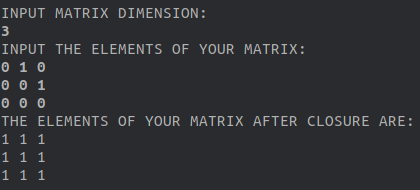
\includegraphics[scale=0.8]{/eq_closure/sample_matrix_output.png}}
	\caption{Матрица бинарного отношения $\delta$ после эквивалентного замыкания.}
\end{figure}

\par Получившееся бинарное отношение $\delta$ является замкнутым относительно
свойств рефлексивности, симметричности и транзитивности, что видно по матрице
этого бинарного отношения. \\

\par \textbf{Оценка временной сложности алгоритма эквивалентного замыкания
  бинарного отношения.}
\par Поскольку алгоритм эквивалентного замыкания использует функции,
реализованные в прошлой лабораторной работе, то воспользуемся уже полученными
оценками: $T(reflexive\_closure, \, n) = O(n\log n), \; T(symmetric\_closure, \,
n) = O(n^2 \log n), \; T(transitive\_closure, n) = O(n^4 \log n).$ Операции
замыкания применяются последовательно, значит, $T(equivalence\_closure, \, n) =
O(n\log n + n^2 \log n + n^4 \log n) = O(n^4 \log n)$.

\newpage

\subsection{Алгоритм нахождения системы представителей по заданному бинарному
  отношению}

\par \textbf{Описание алгоритма нахождения системы представителей по заданному
  бинарному отношению.} \\
\textbf{Вход:} матрица бинарного отношения $\rho.$ \\
\textbf{Выход:} система представителей заданного бинарного отношения $\rho.$ \\
\textbf{Метод:} для получения системы представителей бинарного отношения $\rho$
оно должно являться эквивалентностью. Поэтому сначала бинарное отношение $\rho$
подвергается эквивалентному замыканию. Затем по замкнутому отношению $\rho$
строится фактор-множество этого отношения. Из каждого класса эквивалентности в
построенном фактор-множестве выбирается свой представитель. \\

\par \textbf{Псевдокод алгоритма нахождения системы представителей по заданному
  бинарному отношению.}

\begin{lstlisting}[caption=Псевдокод алгоритма., mathescape]
get_system_of_representatives(<matrix> binaryRelation)
{
  systemOfRepresentatives[], factorSet[[]];
  factorSet[[]] = get_equivalence_classes(binaryRelation);
  for i in range(factorSet.size())
    systemOfRepresentatives.push_back(
                              getRepresentative(factorSet[i]));

  return systemOfRepresentatives;
}
\end{lstlisting}

\par Стоит заметить, что понятию класса эквивалентности в ориентированном графе
соответствует понятие компоненты сильной связности. Для поиска компонент сильной
связности по заданной матрице бинарного отношения используются вспомогательные функции
\textit{get\_equivalence\_classes}, \textit{get\_component\_DFS} и
\textit{order\_DFS}.

\par \textbf{Код программы, реализующей алгоритм нахождения системы
  представителей по заданному бинарному отношению.}

\begin{lstlisting}[caption=Код программы и вспомогательных функций., mathescape]
void orderDFS(vector<vector<int>> adjVector, int vertexNum)
{
  visited[vertexNum] = true;

  for (int i = 0; i < adjVector[vertexNum].size(); ++i)
		if (!visited[adjVector[vertexNum][i]])
      orderDFS(adjVector, adjVector[vertexNum][i]);

  exitOrder.push_back(vertexNum);
}

void getComponentDFS(vector<vector<int>> adjMatrixTransposed,
                     int vertexNum) 
{
  visited[vertexNum] = true;
  component.push_back(vertexNum);

  for (int i = 0; i < adjMatrixTransposed[vertexNum].size(); ++i)
		if (!visited[adjMatrixTransposed[vertexNum][i]])
      getComponentDFS(adjMatrixTransposed,
                      adjMatrixTransposed[vertexNum][i]);
}

vector<vector<int>> getEquivalenceClasses(
  vector<vector<int>> adjMatrix)
{
	int i;
	vector<vector<int>> adjVectorTransposed, connectedComponents;
	vector<vector<int>> adjVector =
    convertMatrixToAdjVector (adjMatrix);
	visited.assign(matrixDimension, false);

	for (i = 0; i < matrixDimension; ++i)
    if (!visited[i])
      orderDFS(adjVector, i);

  adjVectorTransposed =
    convertMatrixToAdjVector (transposeMatrix (adjMatrix));
	visited.assign (matrixDimension, false);
	reverse (exitOrder.begin (), exitOrder.end ());

	for (i = 0; i < matrixDimension; ++i)
	{
		if (!visited[exitOrder[i]])
		{
			getComponentDFS (adjVectorTransposed, exitOrder[i]);
			connectedComponents.push_back (component);
			component.clear ();
		}
	}
  return (connectedComponents);
}

void getSystemOfRepresentatives (vector<vector<int>> adjMatrix)
{
	int i, j;
	vector<int> systemOfRepresentatives;
	vector<vector<int>> connectedComponents =
    getEquivalenceClasses (adjMatrix);

	cout << "FACTOR SET OF THIS BINARY RELATION IS:\n";

	for (i = 0; i < connectedComponents.size (); ++i)
	{
		cout << "{ ";
    for (j = 0; j < connectedComponents[i].size(); ++j)
      cout << connectedComponents[i][j] + 1 <<
        (j == connectedComponents[i].size() - 1 ? " " : ", ");
    cout << "}" <<
      (i == connectedComponents.size() - 1 ? "." : ", ");
  }

	for (i = 0; i < connectedComponents.size(); ++i)
    systemOfRepresentatives.push_back(
      getMin (connectedComponents[i]));

  cout <<
    "\nSYSTEM OF REPRESENTATIVES OF THIS BINARY RELATION IS:\n";

	for (i = 0; i < systemOfRepresentatives.size(); ++i)
    cout << "{ " << systemOfRepresentatives[i] + 1 << " }" <<
      (i == systemOfRepresentatives.size() - 1 ? "." : ", ");
}
\end{lstlisting}

\newpage

\par \textbf{Результат тестирования программы нахождения системы представителей
  по заданной матрице бинарного отношения.}

\par Для демонстрации работы программы рассмотрим бинарное
отношение $\delta$, заданное матрицей.

\par Для заданного бинарного отношения $\delta$ получим систему представителей:

\begin{figure}[h]
	\center{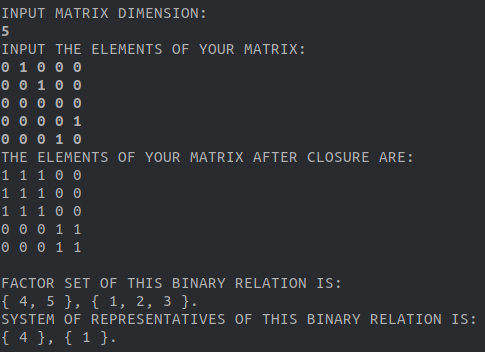
\includegraphics[scale=0.8]{/repr_system/repr_system_output.png}}
	\caption{Система представителей бинарного отношения $\delta$.}
\end{figure}

\par Программа сначала осуществила эквивалентное замыкание заданного бинарного
отношения $\delta$, затем построила фактор-множество и выбрала представителя из
каждого класса эквивалентности. \\

\newpage

\par \textbf{Оценка временной сложности алгоритма построения системы
  представителей заданного бинарного отношения.}

Рассмотрим алгоритм выделения компонент сильной связности, при помощи которого
происходит построение фактор-множества:

\begin{enumerate}
\item Запустить серию обходов в глубину графа G, которая возвращает вершины в
  порядке увеличения времени выхода \textbf{tout}, т.е. некоторый список
  \textbf{order}.
\item Построить транспонированный граф $G^T$. Запустить серию обходов в
  глубину этого графа в порядке, определяемом списком \textbf{order} (а
  именно, в обратном порядке, т.е. в порядке уменьшения времени выхода). Каждое
  множество вершин, достигнутое в результате очередного запуска обхода, и будет
  очередной компонентой сильной связности.
\end{enumerate}

Временная сложность такого алгоритма равна $O(m + n)$, поскольку алгоритм
представляет собой два обхода в глубину. Однако после получения списка
\textbf{order}, необходимо построить транспонированный граф $G^T$, что
увеличивает временную сложность алгоритма до $O(n^2)$ (если предварительно не
сохранять транспонированную матрицу бинарного отношения).

\newpage

\subsection{Алгоритм построения диаграммы Хассе по заданному числу}

\par \textbf{Описание алгоритма построения диаграммы Хассе по заданному числу.} \\
\textbf{Вход:} натуральное число $n$ и два символа 'y'/'n', учитывающих само
число $n$ и 1 в качестве делителей. \\
\textbf{Выход:} диаграмма Хассе отношения делимости для делителей заданного
числа $n$, а также минимальные, максимальные и наименьшие, наибольшие элементы
полученного отношения порядка. \\
\textbf{Метод:} сначала необходимо получить все делители рассматриваемого числа
$n$ (с учётом или без учёта 1 и $n$). В множестве делителей найти минимальные
элементы и расположить их на первом уровне диаграммы Хассе. Затем искать
минимальные элементы в множестве делителей без множества элементов,
расположенных на первом уровне диаграммы Хассе (в последующих случаях, --
исключая элементы, расположенные на предыдущих уровнях диаграммы) и расположить
их на втором уровне диаграммы, сохранить связи, указывающие на отношения делимости
между уровнями диаграммы. Повторять процедуру, пока множество делителей не будет
пусто. Для определения того, какие элементы являются минимальными, максимальными и
наименьшими, наибольшими, просматриваются самый верхний и самый нижний уровень
диаграммы Хассе. Если только один элемент содержится на нижнем
уровне диаграммы Хассе, то он будет и минимальным, и наименьшим. Если же на
нижнем уровне содержится более одного элемента, то наименьший элемент 
отсутствует, а минимальными будут являться все элементы, расположенные на
нижнем уровне. Аналогичные рассуждения проводятся для верхнего уровня и для
максимального и наибольшего элемента.\\

\par \textbf{Псевдокод алгоритма построения диаграммы Хассе по заданному числу.}

\begin{lstlisting}[caption=Псевдокод алгоритма., mathescape]
division_Hasse_diagram(natural_number)
{
  divisors[] = get_divisors(natural_number);
  currentMins[], HasseDiagram[[]];
  
  while (!divisors.empty())
  {
    currentMins = get_mins(divisors);
    HasseDiagram.push_back(currentMins);
    remove_elements(divisors, currentMins);
  }
  make_diagram_connections(HasseDiagram);
}
\end{lstlisting}

\par В качестве вспомогательных используются функции \textit{getDivisors},
возвращающая список делителей заданного числа $n$, \textit{getMins},
возвращающая список минимальных (в соответствии с отношением делимости)
делителей числа $n$ на текущей итерации, \textit{removeMins}, удаляющая из
множества делителей множество минимальных делителей, полученных на текущей
итерации, а также \textit{getHasseConnections}, формирующая связи между
уровнями диаграммы Хассе. \\

\par \textbf{Код программы построения диаграммы Хассе по заданному числу.}

\begin{lstlisting}[caption=Код программы., mathescape]
vector<int> getDivisors(int numberX)
{
	int i, numberOfDivisors = 0;
	char includeOne = '.', includeX = '.';
	vector<int> divisors;

	for (i = 2; i * i < numberX; ++i)
		if (numberX % i == 0)
			++numberOfDivisors;

	while (includeOne != 'y' && includeOne != 'n')
	{
		cout << "INCLUDE ONE ? (y/n):\n";
		cin >> includeOne;
	}
	if (includeOne == 'y')
		divisors.push_back(1);
	while (includeX != 'y' && includeX != 'n')
	{
		cout << "INCLUDE " << numberX << " ? (y/n):\n";
		cin >> includeX;
	}
	if (includeX == 'y')
		divisors.push_back(numberX);
	if (numberOfDivisors == 0 && 
      includeOne == 'n' && 
      includeX == 'n')
	{
		cout << "YOU CAN'T REMOVE THE NUMBER ITSELF 
      AND NUMBER ONE FOR A PRIME NUMBER.";
		exit(0);
	}

	for (i = 2; i <= numberX / 2; ++i)
		if (numberX % i == 0)
			divisors.push_back(i);

	return (divisors);
}

vector<int> getMins(vector<int> divisors)
{
	int i;
	map<int, vector<int>> divisibilityRelation;
	vector<int> mins;

	for (int divisor : divisors)
	{
		vector<int> placeholder;
		divisibilityRelation[divisor] = placeholder;
	}
	for (int divisor : divisors)
	{
		for (int divisorToCheck : divisors)
			if (divisor != divisorToCheck && 
          divisorToCheck % divisor == 0)
				divisibilityRelation[divisor].push_back(divisorToCheck);
	}
	for (int divisor : divisors)
	{
		bool found = false;
		for (auto divisElements : divisibilityRelation)
			for (i = 0; i < divisElements.second.size(); ++i)
			{
				if (divisor == divisElements.second[i])
				{
					found = true;
					break;
				}
				if (found)
					break;
			}
		if (!found)
			mins.push_back(divisor);
	}
	return (mins);
}

void removeMins (vector<int>& divisors, vector<int> mins)
{
	int i;

	for (int min : mins)
	{
		auto it = divisors.cbegin();

		for (i = 0; i < divisors.size(); ++i)
			if (divisors[i] == min)
				divisors.erase (it + i);
	}
}

void getHasseConnectionsMachinerie(
  vector<vector<pair<int, int>>>& HasseLevelConnections, 
  vector<int> lowerLevel, vector<int> upperLevel)
{
	int i;
	vector<pair<int, int>> levelRelations;

	for (int lowerLevelElt : lowerLevel)
	{
		for (int upperLevelElt : upperLevel)
			if (upperLevelElt % lowerLevelElt == 0)
				levelRelations.push_back(
          make_pair(lowerLevelElt, upperLevelElt));
	}
	HasseLevelConnections.push_back(levelRelations);
}

vector<vector<pair<int, int>>> getHasseConnections(
  vector<vector<int>> HasseLevels)
{
	int i;
	vector<vector<pair<int, int>>> HasseLevelConnections;

	for (i = 0; i < HasseLevels.size() - 1; ++i)
		getHasseConnectionsMachinerie(
      HasseLevelConnections, 
      HasseLevels[i], HasseLevels[i + 1]);

	return (HasseLevelConnections);
}

void HasseDiagram ()
{
	int numberX, i;
	vector<int> divisors, mins;
	vector<vector<int>> HasseLevels;
	vector<vector<pair<int, int>>> HasseLevelConnections;

	cout << "INPUT YOU NUMBER:\n";
	cin >> numberX;

	divisors = getDivisors (numberX);

	while (!divisors.empty ())
	{
		mins = getMins (divisors);
		HasseLevels.push_back (mins);
		removeMins (divisors, mins);
	}
	HasseLevelConnections = getHasseConnections (HasseLevels);
	printHasseDiagram (HasseLevels, HasseLevelConnections);
}
\end{lstlisting}

\newpage

\par \textbf{Результат тестирования программы нахождения диаграммы Хассе по
  заданному числу.}

\par Для демонстрации работы программы рассмотрим её выход для заданного числа
60. Само число 60 не будем включать в множество делителей.

\begin{figure}[h]
	\center{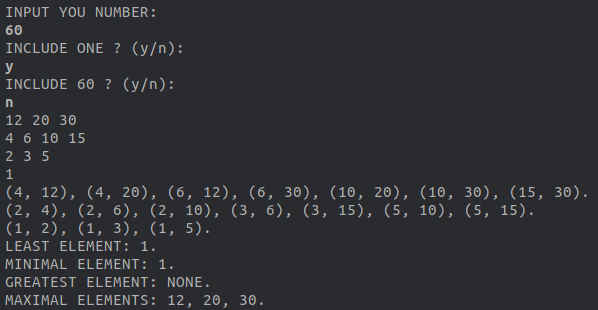
\includegraphics[scale=0.8]{/hasse_diag/number_wo_output.png}}
	\caption{Построение диаграммы Хассе отношения делимости для делителей числа 60
    (без учёта самого числа 60).}
\end{figure}

\par В качестве выхода работы программы была сформирована диаграмма Хассе
отношения делимости на множестве делителей числа 60 (без учёта самого числа 60).
Ниже идут пары вида $(x, y)$, указывающие на связь элементов между уровнями
диаграммы. Также, поскольку само число 60 не рассматривалось как делитель, то
наибольший элемент отсутствует, в то время как максимальными элементами являются
элементы, расположенные на верхнем уровне диаграммы. \\

\par \textbf{Оценка временной сложности алгоритма построения диаграммы Хассе по
  заданному числу.}
\par Сначала в соответствии с псевдокодом рассмотрим операцию получения всех
делителей заданного числа $n$. Для числа $n$ необходимо
проверить, делят ли его все числа от 2 до $n / 2$ (рассмотрение 1 и $n$ зависит
от ввода пользователя). Таким образом, операция получения делителей числа $n$
имеет сложность: $O(n / 2) = O(n)$.

\par Перейдём к рассмотрению содержимого цикла \textit{while}. Первая операция
-- получение минимальных элементов относительно отношения делимости в текущем
множестве делителей. В нашем случае для каждого делителя $d_i$ из множества
делителей $D$ числа $n$ ищется элемент $d_j$ из множества $D$ такой, что $d_j$
делит $d_i$. Если такой элемент $d_j$ для элемента $d_i$ не найден, то $d_i$
признаётся минимальным в текущем множестве делителей. Поскольку поиск такого
делителя $d_j$ для $d_i$ осуществляется проходом по текущему множеству
делителей, то $T(get\_mins, n) = O(|D|^2)$, где $|D|$ -- мощность множества
делителей заданного числа $n$.

\par Следующая операция -- удаление найденных на текущей итерации минимальных
элементов из множества делителей. Достигается путём поиска соответствющих
элементов в множестве делителей и их удалении оттуда. Сложность операции: $O(|D|^2)$.

\par В худшем случае цикл \textit{while} будет выполняться $|D|$ раз -- в
случае, если диаграмма Хассе представляет собой цепь. Тогда временная сложность
содержимого цикла составляет: $T(while(), n) = O(|D|(|D|^2 + |D|^2)) =
O(|D|^3)$, где $|D|$ -- мощность множества делителей заданного числа $n$.

\par Последняя операция (функция \textit{makeDiagramConnections}) отвечает
за процесс формирования связей между уровнями диаграммы Хассе. Операция
выполняется следующим образом: между каждыми двумя смежными уровнями диаграммы
Хассе формируются связи, соответствующие отношению делимости между элементами
этих уровней. Для каждого элемента нижнего уровня просматриваются все элементы
верхнего уровня и выполняется проверка на то, делит ли элемент нижнего уровня
элемент верхнего уровня. Если да, то факт наличия связи между двумя
рассматриваемыми элементами сохраняется в контейнере связей.

\par Получим оценку временной сложности этой операции. Будем считать, что 1 и
$n$ учитывается в множестве делителей. Предположим, что ранее была сформирована
диаграмма Хассе с $p$ уровнями. Через $n_i$ ($i = 1,\dots, p$) обозначим число элементов на каждом
уровне диаграммы Хассе. Очевидно, что $ \sum_{i = 1}^{p} n_i = |D| $, где
$|D|$ -- мощность множества делителей заданного числа $n$. Тогда общее число
операций, совершаемое функцией \textit{makeDiagramConnections} составляет $
\sum_{i = 1}^{p - 1} n_i n_{i + 1}$. Определим $N = \max n_i, \, i = 1,\dots,p
$. Заметим, что $n_i \leq N \leq |D| \; \text{и} \; p \leq |D|$. Оценим число операций
функции \textit{makeDiagramConnections} сверху: $$ \sum_{i = 1}^{p -
  1}n_in_{i + 1} \leq \sum_{i = 1}^{p - 1}N^2 = N^2 \sum_{i = 1}^{p - 1} 1 \leq
N^2 (p - 1) \leq |D|^3.$$

\par Тогда, общая временная оценка алгоритма построения диаграммы Хассе по
заданному числу: $T(Hasse\_diagram, n) = O(n + |D|^3 + |D|^3) = O(n + |D|^3)$,
где $|D|$ -- мощность множества числа делителей заданного числа n.

\newpage

\subsection{Алгоритм построения диаграммы Хассе по заданной матрице порядка}

\par \textbf{Описание алгоритма построения диаграммы Хассе по заданной матрице
  порядка.} \\
\textbf{Вход:} матрица порядка бинарного отношения $\rho$. \\
\textbf{Выход:} диаграмма Хассе заданного бинарного отношения порядка $\rho$. \\
\textbf{Метод:} сначала формируется контейнер, содержащий элементы заданного отношения
порядка. Затем, пока этот контейнер не пуст, осуществляется поиск минимальных
элементов отношения порядка по заданной матрице. В матрице минимальному элементу
отношения порядка соответствует такой элемент, что его столбец не содержит
единиц, кроме как на позиции, где $i$ равен $j$ (номер строки совпадает с
номером столбца -- в силу рефлексивности отношения порядка). Найденные на первой
итерации минимальные элементы составляют первый уровень диаграммы Хассе. После,
эти минимальные элементы должны быть убраны из контейнера и поиск минимальных
элементов теперь осуществляется в обновлённом контейнере. Найденные на второй
итерации минимальные элементы будут составлять второй уровень диаграммы Хассе и
т.д.. После составления диаграммы Хассе необходимо сформировать связи между
элементами уровней диаграммы. Для этого рассматриваются каждые два смежных
уровня получившейся диаграммы Хассе. Для каждого элемента нижнего уровня в
матрице порядка ищутся элементы верхнего уровня, с которыми он состоит в
отношении порядка. Соответствующие связи добавляются в контейнер связей. \\

\par \textbf{Псевдокод алгоритма построения диаграммы Хассе по заданной матрице порядка.}

\begin{lstlisting}[caption=Псевдокод алгоритма., mathescape]
Hasse_diagram_matrix(<matrix> orderBinaryRelation)
{
  eltContainer[] = get_elements(orderBinaryRelation);
  HasseDiagram[[]], mins[];

  while (!eltContainer.empty())
  {
    mins = get_min_elts(matrix, eltContainer);
    HasseDiagram.push_back(mins);
    remove_mins (orderBinaryRelation, eltContainer, mins);
  }
  HasseDiagram = getHasseConnectionsMatrix(
                   HasseDiagram, orderBinaryRelation);
}
\end{lstlisting}

\par В качестве вспомогательных используются функции \textit{getMinsMatrix},
извлекающая на текущей итерации минимальные элементы отношения порядка,
\textit{removeMinElts}, удаляющая из контейнера \textit{elements} минимальные
элементы, найденные на текущей итерации, \textit{cleanRows}, выполняющая
аналогичную функцию, но для матрицы порядка, и
\textit{getHasseConnectionsMatrix}, выполняющая построение связей между уровнями
диаграммы Хассе.
\\
\par \textbf{Код программы построения диаграммы Хассе по заданной матрице порядка.}

\begin{lstlisting}[caption=Код программы., mathescape]
void cleanRows (vector<vector<int>>& matrix, vector<int> mins)
{
	int i;

	for (int min : mins)
		for (i = 0; i < matrixDimension; ++i)
			if (matrix[min][i] == 1)
				matrix[min][i] = 0;
}

void removeMinElts (vector<int>& elts, vector<int> mins)
{
	int i;

	for (int min : mins)
	{
		auto it = elts.cbegin ();
		for (i = 0; i < elts.size (); ++i)
			if (elts[i] == min)
				elts.erase (it + i);
	}
}

bool inElements (vector<int> elements, int i)
{
	int j;

	for (j = 0; j < elements.size (); ++j)
		if (elements[j] == i)
			return (true);

	return (false);
}

vector<int> getMinsMatrix (vector<vector<int>> matrix,
                           vector<int> elements)
{
	int i, j;
	vector<int> mins;

	for (i = 0; i < matrixDimension; ++i)
	{
		bool isMin = true;

		for (j = 0; j < matrixDimension; ++j)
			if (matrix[j][i] == 1 && i != j)
			{
				isMin = false;
				break;
			}
		if (isMin && inElements (elements, i))
			mins.push_back (i);
	}
	return (mins);
}

void getHasseConnectionsMatrix (
  vector<vector<int>> matrix, 
  vector<int> pLevel, vector<int> nLevel,
  vector<vector<pair<int, int>>>& levelsConnections)
{
	int i, j;
	vector<pair<int, int>> levelConnections;

	for (int pLvlElt : pLevel)	
		for (int nLvlElt : nLevel)
			if (matrix[pLvlElt][nLvlElt] == 1)
				levelConnections.push_back (
          make_pair (pLvlElt + 1, nLvlElt + 1));	

	levelsConnections.push_back (levelConnections);
}

void HasseDiagramMatrix ()
{
	int i;
	vector<vector<int>> matrix, matrixCopy, HasseLevels;
	vector<vector<pair<int, int>>> HasseLevelConnections;
	vector<int> elements, mins;
	cout << "INPUT MATRIX DIMENSION:\n";
	cin >> matrixDimension;

	getMatrix (matrix);

	matrixCopy = matrix;

	for (i = 0; i < matrix.size (); ++i)
		elements.push_back (i);

	while (!elements.empty ())
	{
		mins = getMinsMatrix (matrix, elements);
		HasseLevels.push_back (mins);
		removeMinElts (elements, mins);
		cleanRows (matrix, mins);
	}

	for (i = 0; i < HasseLevels.size () - 1; ++i)	
		getHasseConnectionsMatrix (
      matrixCopy, HasseLevels[i], 
      HasseLevels[i + 1], HasseLevelConnections);

	displayLevelsAndConnections (HasseLevels,
                                 HasseLevelConnections);
}
\end{lstlisting}

\newpage

\par \textbf{Результат тестирования программы построения диаграммы Хассе по
  заданной матрице порядка.}

\par Рассмотрим отношение порядка $\delta$, заданное матрицей. Построим
диаграмму Хассе для рассматриваемого отношения порядка:

\begin{figure}[h]
  \center{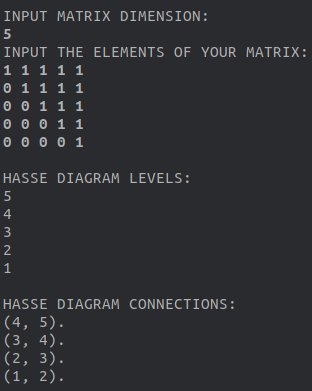
\includegraphics[scale=0.8]{/hasse_diag_mat/chain.png}}
  \caption{Диаграмма Хассе заданного отношения порядка $\delta$.}
\end{figure}

\par Как видно, построенная диаграмма Хассе для заданного отношения порядка $\delta$
является \textit{цепью}.
\\
\par \textbf{Оценка временной сложности алгоритма построения диаграммы Хассе по
  заданной матрице порядка.}

\par В соответствии с псевдокодом будем последовательно рассматривать сложность
каждой из выполняемых операций.

\par Первая операция -- формирование контейнера
элементов. Сложность операции: $O(n)$, т.к. должен быть учтён каждый уникальный
элемент, участвующий в отношении порядка, где $n$ -- размерность входной
квадратной матрицы порядка. 

\par Далее будем рассматривать операции, выполняемые внутри цикла
\textit{while}. Первая операция внутри цикла -- поиск минимальных элементов
отношения порядка на текущей итерации. В качестве примера рассмотрим число
совершаемых операций на первой итерации, т.е. во время поиска первых минимальных
элементов отношения порядка. Т.к. для определения того, является ли
элемент минимальным, необходимо полностью просмотреть его столбец в матрице
порядка, то для нахождения всех минимальных элементов на
первой итерации необходимо осуществить $n^2$ операций. На следующих итерациях,
когда минимальные элементы предыдущих итераций рассматривать уже не надо, число
операций будет уменьшаться, однако верхняя граница в $n^2$ операций (где $n^2$
-- число элементов в исходной матрице порядка) по-прежнему будет верна. Таким
образом, $T(getMinsMatrix, n) = O(n^2)$.

\par Вторая операция внутри цикла -- удаление минимальных элементов из
контейнера и обновление значений в матрице. Для того, чтобы удалить минимальное
значение из контейнера, его сначала необходимо найти. После нахождения нужного
значения оно удаляется. Верхняя граница сложности такой операции: $O(n^2)$,
поскольку на первой итерации все элементы могут оказаться минимальными, и
придётся осуществлять поиск каждого элемента в контейнере. В случае с матрицей
строка элемента, являющегося минимальным на текущей итерации заполняется нулями.
Таким образом, верхняя граница сложности такой операции: $O(n^2)$.

\par Поскольку на каждом шаге выполнения алгоритма находится как минимум один
минимальный элемент (при корректных входных данных), то условие
\textit{while (!eltContainer.empty())} может быть выполнено максимум $n$ раз,
где $n$ -- число строк или столбцов в исходной квадратной матрице порядка. Таким
образом верхняя граница сложности рассматриваемого цикла: $T(while(), n) = O(n^3)$.

\par После выполнения цикла необходимо сформировать связи между уровнями
диаграммы Хассе. Для этого рассматриваются каждые два смежных уровня в диаграмме
Хассе. Для каждого элемента нижнего уровня рассматривается каждый элемент
верхнего уровня и ищется значение в матрице (в копии матрицы, т.к. после
построения диаграммы Хассе исходная матрица порядка -- нулевая), стоящее на пересечении
соответствующих строки и столбца. Если значение -- единица, то в
контейнер связей добавляется отношение между соответствующими элементами (пара
этих элементов).

\par Допустим, что после построения диаграмма Хассе содержит $p$
уровней. Через $n_i \, (i = 1,\dots,p)$ обозначим число элементов на каждом
уровне. Очевидно, что $\sum_{i = 1}^{p} n_i = n$, где $n$ -- число строк или
столбцов в исходной квадратной матрице порядка. Тогда число операций, которое
необходимо выполнить для формирования связей между уровнями диаграммы Хассе в
соответствии с описанием процедуры: $\sum_{i = 1}^{p - 1} n_i n_{i + 1}$.
Обозначим $N = \max n_i \, (i = 1,\dots,p).$ Также видно, что $n_i \leq N \leq
n$ и $p \leq n$. Тогда: $$ \sum_{i = 1}^{p - 1} n_i n_{i + 1} \leq N^2 \sum_{i =
  1}^{p - 1} 1 = N^2 (p - 1) \leq n^3$$

\par Таким образом, временная сложность
алгоритма построения диаграммы Хассе по заданной матрице порядка составляет:
$T(Hasse\_diagram\_matrix, n) = O(n + n(n^2 + n^2) + n^3) = O(n^3).$

\newpage

\subsection{Алгоритм построения решётки концептов}
\par \textbf{Описание алгоритма построения решётки концептов.} \\
\textbf{Вход:} контекст $K$ (множество объектов $G$, множество атрибутов $M$,
бинарное отношение $\rho \subset G \times M$). \\
\textbf{Выход:} решётка концептов $C(K)$ и её диаграмма Хассе. \\
\textbf{Метод:} сначала вычисляется система замыканий $Z_{f_G}$ на множестве
$G$ и строится её диаграмма Хассе. Затем составляется решётка концептов $C(K)$,
формируются связи между уровнями диаграммы Хассе. Полученная диаграмма Хассе
дополняется элементами из решётки концептов. Система замыканий $Z_{f_G}$ строится путём
вычисления $\rho^{-1}(a_i), \, a_i \in M \, (i = 1,\dots,|M|)$, добавления его в
$Z_{f_G}$ и попарного пересечения получившегося множества $\rho^{-1} (a_i)$ с
уже имеющимися в
$Z_{f_G}$ множествами и их последующего добавления в $Z_{f_G}$. Диаграмма Хассе
системы замыканий $Z_{f_G}$ строится на основе отношения
теоретико-множественного включения. Для поиска минимальных элементов в $Z_{f_G}$
для каждого элемента (множества) из $Z_{f_G}$ на каждой итерации алгоритма
построения диаграммы Хассе будем хранить набор множеств из $Z_{f_G}$,
содержащихся в рассматриваемом множестве. Таким образом, если рассматриваемое
множество не содержит в себе ни одного элемента (множества) из $Z_{f_G}$, кроме
самого себя, то оно является минимальным элементом на текущей итерации
построения диаграммы Хассе. Минимальные элементы, полученные на первой итерации
алгоритма построения диаграммы Хассе представляют собой первый уровень
диаграммы. Для построения второго уровня диаграммы из системы замыканий $Z_{f_G}$
необходимо удалить минимальные элементы, найденные на первой итерации алгоритма
построения диаграммы Хассе и повторить процедуру построения содержащихся наборов
множеств. Алгоритм будет выполняться и формировать новые уровни диаграммы Хассе,
пока $Z_{f_G}$ не станет пустым. После построения диаграммы связи между уровнями
формируются следующим образом: для каждых двух смежных уровней диаграммы для
каждого элемента (множества) нижнего уровня проверяется факт его включения в
элементы (множества) верхнего уровня. Пара
элементов (множеств), для которых это условие выполняется, заносится в контейнер
связей. После построения диаграммы Хассе и формирования её связей, в дополнение
к каждому элементу (множеству объектов) каждого уровня диаграммы ставится в
соответствие элемент (множество атрибутов) решётки концептов -- набор общих
атрибутов для соответствующего множества объектов.
\\
\par \textbf{Псевдокод алгоритма построения решётки концептов.}

\begin{lstlisting}[caption=Псевдокод алгоритма., mathescape]
get_concept_grid(objectSet[], attrSet[], <matrix> binaryRelation)
{
  mins[[]], HasseDiagram[[[]]], $Z_{f_G}$[[]];
  $Z_{f_G}$ = get_closure_system(objectSet, attrSet, binaryRelation);
  
  while (!$Z_{f_G}.empty()$)
  {
    mins = get_mins(construct_subsets($Z_{f_G}$));
    HasseDiagram.push_back(mins);
    remove_mins($Z_{f_G}$, mins);
  }
  HasseDiagram = get_Hasse_Connections(HasseDiagram);
  HasseDiagram = complete_with_attributes(HasseDiagram);
}
\end{lstlisting}

\par В качестве вспомогательных используются функции \textit{getInverse} и
\textit{getIntersects}, осуществляющие вычисление системы замыканий $Z_{f_G}$,
\textit{getHasseDiagramConceptGrid}, осуществляющая построение диаграммы Хассе
по полученной системе замыканий $Z_{f_G}$, \textit{getSubsetRelation}, которая
осуществляет идею построения набора множеств из $Z_{f_G}$, содержащихся в
некотором множестве из $Z_{f_G}$ для каждого множества из $Z_{f_G}$,
\textit{removeMinsConcept}, осуществляющая удаление минимальных элементов,
найденных на текущей итерации, из $Z_{f_G}$,
\textit{getHasseConnectionsConcept}, формирующая связи между элементами смежных
уровней диаграммы Хассе, \textit{HasseAttributeSet}, ставящая в дополнение к
каждому элементу (множеству объектов) каждого уровня диаграммы Хассе
соответствующий элемент (множество атрибутов) решётки концептов.
\\
\par \textbf{Код программы построения решётки концептов.}
\begin{lstlisting}[caption=Псевдокод алгоритма., mathescape]
void getIntersects (vector<vector<int>>& setGrid)
{
	int i, j;

	for (i = 1; i < setGrid.size (); ++i)
	{
		for (j = 1; j < setGrid.size (); ++j)
		{
			vector<int> intersection = intersect (setGrid[i],
                                            setGrid[j]);

			if (i != j && !inGrid (setGrid, intersection))
				setGrid.push_back (intersection);
		}				
	}
}

void getSubsetRelation (
  map<vector<int>, vector<vector<int>>>& subsetRelation, 
  vector<vector<int>> setGrid)
{
	int i, j;

	for (auto setAndSubsets : subsetRelation)
	{
		vector<vector<int>> subsets;

		for (j = 0; j < setGrid.size (); ++j)
			if (isSubset (setAndSubsets.first, setGrid[j]) && 
          setAndSubsets.first != setGrid[j])
				subsets.push_back (setGrid[j]);
		subsetRelation[setAndSubsets.first] = subsets;
	}
}

vector<vector<int>> getMinsConcept (
  map<vector<int>, vector<vector<int>>> subsetRelation)
{
	int i;
	vector<vector<int>> mins;

	for (auto setAndSubsets : subsetRelation)
	{
		vector<int> set = setAndSubsets.first;

		if (subsetRelation[set].empty ())
			mins.push_back (set);
	}

	return (mins);
}

void removeMinsConcept (
  map<vector<int>, vector<vector<int>>>& subsetRelation, 
  vector<vector<int>>& setGrid, vector<vector<int>> mins)
{
	int i;

	for (vector<int> min : mins)
	{
		auto it = setGrid.cbegin ();

		for (i = 0; i < setGrid.size (); ++i)
			if (setGrid[i] == min)
				setGrid.erase (it + i);
	}
	for (i = 0; i < mins.size (); ++i)
		subsetRelation.erase (subsetRelation.find (mins[i]));
}

vector<char> getAttributeSetConceptMachinerie (
  int objectNum, vector<vector<int>> matrix)
{
	int i;
	vector<char> objectAttributes;

	for (i = 0; i < matrix.size (); ++i)
		if (matrix[objectNum][i] == 1)
			objectAttributes.push_back (attributeSet[i]);
		
	if (objectAttributes.empty ())
		objectAttributes.push_back ('!');

	return (objectAttributes);
}

vector<char> getAttributeSetConcept (
  vector<int> HasseLevelSet, vector<vector<int>> matrix)
{
	int i;
	vector<char> objectAttributeSet;

	if (HasseLevelSet[0] == -1)
		return (attributeSet);

	for (i = 0; i < matrix.size (); ++i)
		if (matrix[HasseLevelSet[0]][i] == 1)
			objectAttributeSet.push_back (attributeSet[i]);

	if (objectAttributeSet.empty ())
	{
		objectAttributeSet.push_back ('!');
		return (objectAttributeSet);
	}

	for (i = 1; i < HasseLevelSet.size (); ++i)
		objectAttributeSet = charIntersect (
      objectAttributeSet, 
      getAttributeSetConceptMachinerie (HasseLevelSet[i], 
                                        matrix));

	if (objectAttributeSet.empty ())
	{
		objectAttributeSet.push_back ('!');
		return (objectAttributeSet);
	}

	return (objectAttributeSet);
}

void HasseAttributeSet (
  vector<vector<vector<int>>> HasseLevels, 
  vector<vector<pair<vector<int>, 
  vector<int>>>> HasseLevelsConnections,
  vector<vector<int>> matrix)
{
	int i, j;
	vector<vector<pair<vector<int>, 
                     vector<char>>>> alignedAttributeSets;

	for (auto HasseLevel : HasseLevels)
	{
		vector<pair<vector<int>, 
           vector<char>>> levelAlignedAttributeSets;

		for (vector<int> set : HasseLevel)
			levelAlignedAttributeSets.push_back (
        make_pair (set, getAttributeSetConcept (set, matrix)));

		alignedAttributeSets.push_back (levelAlignedAttributeSets);
	}
	displayConceptGrid (HasseLevelsConnections, 
                      alignedAttributeSets);
}

vector<pair<vector<int>, 
       vector<int>>> getHasseConnectionsConceptMachinerie (
  vector<vector<int>> pLevel, vector<vector<int>> nLevel)
{
	int i, j;
	vector<pair<vector<int>, vector<int>>> levelConnections;

	for (i = 0; i < pLevel.size (); ++i)
	{
		for (j = 0; j < nLevel.size (); ++j)
			if (isSubset (nLevel[j], pLevel[i]))
				levelConnections.push_back (make_pair (pLevel[i], 
                                               nLevel[j]));
	}
	return (levelConnections);
}

void getHasseConnectionsConcept (
  vector<vector<vector<int>>> HasseLevels, 
  vector<vector<pair<vector<int>, 
                vector<int>>>>& HasseLevelsConnections)
{
	int i;

	for (i = 0; i < HasseLevels.size () - 1; ++i)
		HasseLevelsConnections.push_back (
      getHasseConnectionsConceptMachinerie (
        HasseLevels[i], HasseLevels[i + 1]));
}

void getHasseDiagramConceptGrid (
  vector<vector<int>>& closuredSetGrid, 
  vector<vector<int>> matrix)
{
	int i;
	vector<vector<int>> mins;
	vector<vector<vector<int>>> HasseLevels;
	vector<vector<pair<vector<int>, 
                     vector<int>>>> HasseLevelsConnections;
	map<vector<int>, vector<vector<int>>> subsetRelation;

	for (i = 0; i < closuredSetGrid.size (); ++i)
	{
		vector<vector<int>> subsets;
		subsetRelation[closuredSetGrid[i]] = subsets;
	}

	while (!closuredSetGrid.empty ())
	{
		getSubsetRelation (subsetRelation, closuredSetGrid);
		mins = getMinsConcept (subsetRelation);
		HasseLevels.push_back (mins);
		removeMinsConcept (subsetRelation, closuredSetGrid, mins);
	}
	getHasseConnectionsConcept (HasseLevels, 
                              HasseLevelsConnections);
	HasseAttributeSet (HasseLevels, 
                     HasseLevelsConnections, 
                     matrix);
}

void getInverse (vector<vector<int>> matrix, 
                 vector<vector<int>>& closuredSetGrid)
{
	int i, j;
	vector<int> inverseRow;

	for (i = 0; i < matrixDimension; ++i)
		inverseRow.push_back (i);

	closuredSetGrid.push_back (inverseRow);
	inverseRow.clear ();

	for (i = 0; i < matrixDimension; ++i)
	{
		for (j = 0; j < matrixDimension; ++j)
			if (matrix[j][i] == 1)
				inverseRow.push_back (j);

		if (closuredSetGrid[0] != inverseRow)
			closuredSetGrid.push_back (inverseRow);

		inverseRow.clear ();
	}

	getIntersects (closuredSetGrid);
}

void conceptGrid ()
{
	vector<int> objectSet;
	vector<vector<int>> matrix;
	vector<vector<int>> closuredSetGrid;

	cout << "INPUT MATRIX DIMENSION\n";
	cin >> matrixDimension;

	cout << "INPUT YOUR OBJECTS:\n";
	getObjectSet (objectSet);

	cout << "INPUT YOUR ATTRIBUTES:\n";
	getAttributeSet ();
	getMatrix (matrix);

	getInverse (matrix, closuredSetGrid);
	getHasseDiagramConceptGrid (closuredSetGrid, matrix);
}
\end{lstlisting}

\newpage

\par \textbf{Результат тестирования программы построения решётки концептов.}

\par Рассмотрим контекст $K$ с множеством объектов $G = \{1, 2, 3, 4\}}$,
множеством атрибутов $M = \{a, b, c, d\}$ и отношением $\rho$, определяемым матрицей.

\begin{figure}[h]
	\center{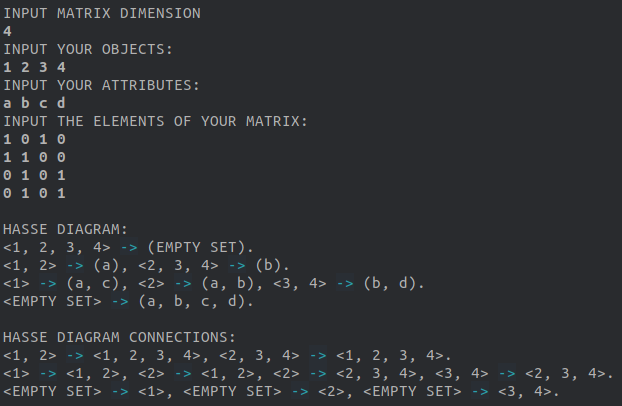
\includegraphics[scale=0.75]{/concept/grid_example.png}}
	\caption{Диаграмма Хассе решётки концептов $C(K)$ заданного контекста K,
    изоморфная диаграмме системы замыканий $Z_{f_G}$.}
\end{figure}

\par Результатом работы программы является вывод построенной для решётки
концептов $C(K)$ диаграммы Хассе по уровням, а также вывод сформированных между
элементами уровней связей.
\\
\par \textbf{Оценка временной сложности алгоритма построения решётки концептов.}
\par Для оценки временной сложности алгоритма будем рассматривать сложность
каждой реализуемой им операции в соответствии с псевдокодом.

\par Первая операция -- построение системы замыканий $Z_{f_G}$ на множестве $G$.
Изначально в $Z_{f_G}$ кладётся само множество $G$, затем вычисляются значения
$\rho^{-1} (a_i), \, i = 1,\dots,|M|, \, \rho \subset G \times M $ -- заданное
бинарное отношение. Для вычисления значения $\rho^{-1} (a_i)$ необходимо
осуществить проход по столбцу соответствующего атрибута $a_i$. Тогда число
операций, необходимое для вычисления промежуточного значения системы замыканий
$Z_{f_G}$ составляет $n^2$, где $n$ -- число строк или столбцов в квадратной
матрице бинарного отношения $\rho$. Для получения полной системы 
замыканий $Z_{f_G}$ каждый элемент промежуточного значения системы $Z_{f_G}$
пересекается со всеми остальными элементами в $Z_{f_G}$, и полученные новые
множества добавляются в $Z_{f_G}$. Заметим, что после построения $Z_{f_G}$
верно, что $|Z_{f_G}| \leq |2^G|$ -- мощность булеана множества объектов $G$.
Грубо оценим сверху число необходимых операций для построения системы замыканий
$Z_{f_G}$ как $|2^G| \cdot |2^G| \cdot n^2$, где $n^2$ -- верхняя граница числа
операций, необходимых для выполнения пересечения двух множеств (мощность каждого
множества не превосходит $n$). $|2^G|$ может быть заменено на $2^n$, тогда:
$T(get\_closure\_system, n) = O(2^n \cdot 2^n \cdot n^2 + n^2) = O(n^2 \cdot 4^n)$, где $n$
-- число строк или столбцов в квадратной матрице заданного бинарного отношения
$\rho$.

\par Перейдём к рассмотрению операций, выполняемых внутри цикла $while$. Первая
операция -- поиск минимальных элементов на текущей итерации в системе замыканий
$Z_{f_G}$. Для этого для каждого элемента (множества) из $Z_{f_G}$ хранится набор множеств
из $Z_{f_G}$, содержащихся в рассматриваемом множестве. Для построения такого
набора необходимо зафиксировать некоторый элемент (множество) из $Z_{f_G}$ и для оставшихся
в $Z_{f_G}$ множеств проверить, являются ли они подмножествами зафиксированного
элемента. Поскольку мощность каждого элемента $Z_{f_G}$ не превосходит $n$ ($n$
-- мощность множества объектов или множества атрибутов), то верхней границей
числа операций, необходимых для определения того, является ли рассматриваемое
множество из $Z_{f_G}$ подмножеством фиксированного элемента, будет $n^2$.
Также, поскольку $|Z_{f_g}| \leq |2^G| = 2^n$, временная оценка сложности операции поиска
минимальных элементов на текущей итерации принимает вид: $T(get\_mins, n) =
O(n^2 \cdot 4^n)$.

\par Следующая операция -- удаление найденных минимальных элементов из системы
замыканий $Z_{f_G}$. Здесь будут действовать те же самые оценки временной
сложности, полученные для предыдущих операций, за исключением того, что не будет
производиться дополнительных процедур с временной сложность $O(n^2)$, поэтому:
$T(remove\_mins, n) = O(4^n)$. 

\par Поскольку две рассмотренные выше операции выполняются внутри цикла, который
может выполняться не более $2^n$ раз, то общая временная сложность операции с
циклом составляет: $T(while(), n) = O(2^n \cdot (n^2 \cdot 4^n + 4^n)) = O(n^2
\cdot 8^n)$.

\par Следующая операция -- построение связей между элементами разных уровней
диаграммы Хассе. Будем считать, что была сформирована диаграмма Хассе с $p$
уровнями. Через $n_i$ обозначим число элементов на каждом уровне диаграммы
Хассе, $i = 1,\dots,p$. Очевидно, что $\sum_{i = 1}^{p} n_i = |Z_{f_G}|.$
Обозначим через $n_{ij}$ $j$-ый элемент $i$-го уровня $(j = 1,\dots,n_i, \; i =
1,\dots,p)$. Будем считать, что между элементами должна быть сформирована связь,
если $n_{ij} \subset n_{i + 1k} \, (i = 1,\dots,p - 1, \, j = 1,\dots,n_i, \, k =
1,\dots,n_{i + 1})$. Тогда число операций, необходимое для формирования связей
между элементами уровней диаграммы Хассе не превосходит $\sum_{i = 1}^{p - 1}
n_i n_{i + 1} \cdot \max\limits_{j = 1,\dots,n_i} |n_{ij}| \cdot \max\limits_{k
  = 1,\dots,n_{i + 1}} |n_{i + 1k}|$. Т.к. $n_i \leq \max\limits_{i = 1,\dots,p}
n_i \leq |Z_{f_G}| \leq |2^G| = 2^n$ и $\max\limits_{j = 1,\dots,n_i} |n_{ij}|
\leq n$ и $p \leq |Z_{f_G}| \leq |2^G| = 2^n$, то $\sum_{i = 1}^{p - 1}
n_i n_{i + 1} \cdot \max\limits_{j = 1,\dots,n_i} |n_{ij}| \cdot \max\limits_{k
  = 1,\dots,n_{i + 1}} |n_{i + 1k}| \leq n^2 \cdot 4^n \sum_{i = 1}^{p - 1} 1
\leq n^2 \cdot 8^n.$ Таким образом, оценка временной сложности операции
формирования связей между элементами уровней диаграммы Хассе:
$T(get\_Hasse\_connections, n) = O(n^2 \cdot 8^n).$

\par Последняя операция -- дополнение каждого элемента диаграммы Хассе
соответствующим элементом решётки концептов $C(K)$ заданного контекста $K$. Т.к.
необходимо дополнить каждый элемент системы замыканий $Z_{f_G}$, которых не
более, чем $2^n$, множеством из решётки концептов, которое представляет собой
пересечение не более, чем $n$ множеств (с операцией пересечения, требующей не
более $n^2$ шагов), то оценка временной сложности операции дополнения каждого
элемента диаграммы Хассе принимает вид: $T(complete\_with\_attributes, n) = O(n^3
\cdot 2^n).$

\par Тогда оценка временной сложности алгоритма построения решётки концептов:
$T(get\_concept\_grid, n) = O(n^2 \cdot 4^n + n^2 \cdot 8^n + n^3 \cdot 2^n) =
O(n^2 \cdot 8^n)$, где $n$ -- мощность множества объектов или множества атрибутов.

\newpage

\conclusion

\par В ходе лабораторной работы мною были изучены основные свойства бинарных
отношений и операций их замыкания. В качестве практического задания мною были
описаны и реализованы алгоритмы построения эквивалентного замыкания бинарного
отношения, алгоритм построения фактор-множества, нахождения минимальных,
наименьшего и максимальных, наибольшего элементов в заданном отношении порядка,
алгоритм построения диаграммы Хассе для отношения делимости по заданному
натуральному числу, алгоритм построения диаграммы Хассе по заданной матрице
порядка, а также алгоритм построения диаграммы Хассе решётки концептов по заданному контексту.
Для этих алгоритмов были представлены псевдокоды, осуществлена их программная
реализация, а также проведена оценка временной сложности.

\end{document}

\begin{lstlisting}[caption=Псевдокод алгоритма., mathescape]
get_concept_grid(objectSet[], attrSet[], <matrix> binaryRelation)
{
  mins[[]], HasseDiagram[[[]]], $Z_{f_G}$[[]];
  $Z_{f_g}$ = get_closure_system(objectSet, attrSet, binaryRelation);
  
  while (!$Z_{f_g}.empty()$)
  {
    mins = get_mins(construct_subsets($Z_{f_g}$));
    HasseDiagram.push_back(mins);
    remove_mins($Z_{f_g}$, mins);
  }
  HasseDiagram = get_Hasse_Connections(HasseDiagram);
  HasseDiagram = complete_with_attributes(HasseDiagram);
}
\end{lstlisting}



















